\hypertarget{des-simulation}{%
\section{DES Simulation}\label{des-simulation}}

\begin{figure}
\centering
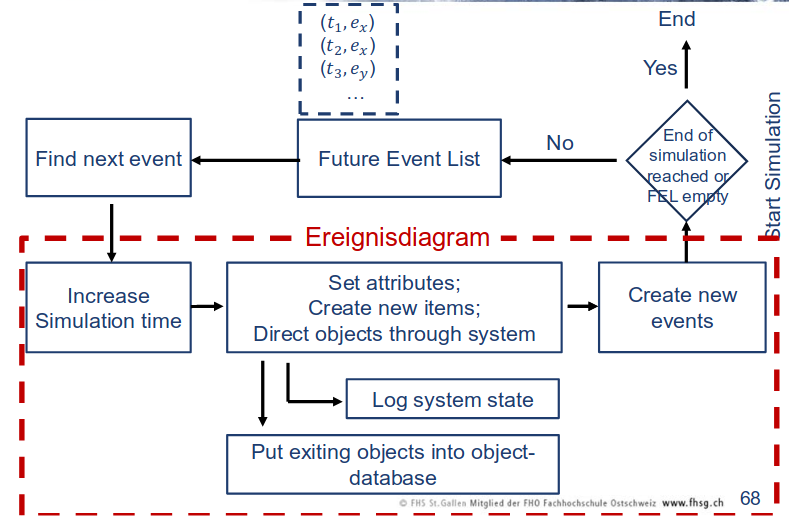
\includegraphics{figures/ereignisdiagram.png}
\caption{Eriegnisdiagramm}
\end{figure}

\hypertarget{de-mechanics}{%
\subsection{DE Mechanics}\label{de-mechanics}}

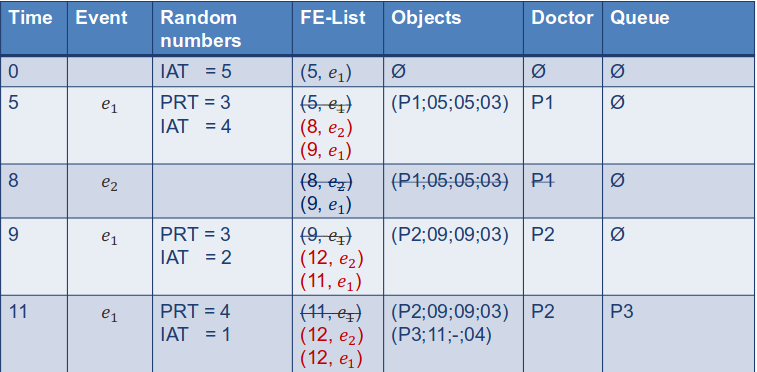
\includegraphics{figures/DEMech1.png}
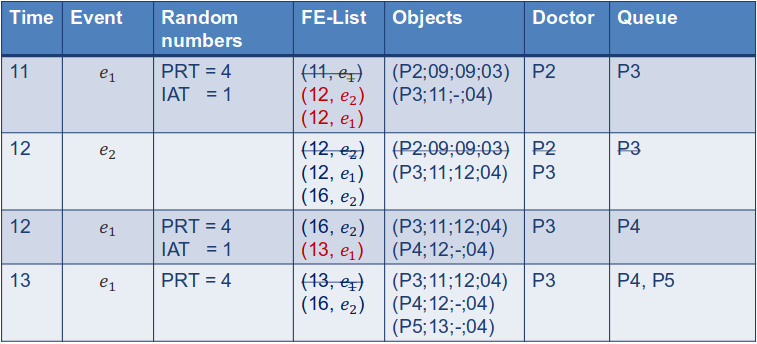
\includegraphics{figures/DEMech2.png}
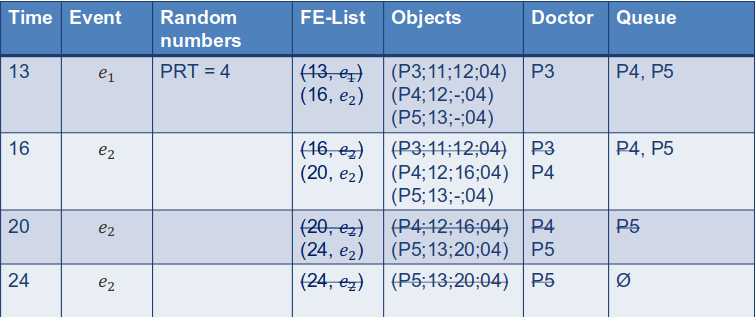
\includegraphics{figures/DEMech3.png}

\begin{itemize}
\tightlist
\item
  PRT = Process Time (Zeit wie lange die Behndlung/Prozess dauert)
\item
  IAT = Inter arrival time (Zeit bis nächster Event eintrift)
\item
  FE-List = Time of next event
\item
  Objects = Current Working state
\item
  Queue = Waiting list
\end{itemize}

\hypertarget{stochastic-processes}{%
\subsection{Stochastic processes}\label{stochastic-processes}}

When modeling processes random variables are often use to define PRTs
and IATs or any other value.

\hypertarget{random-variables}{%
\subsubsection{Random variables}\label{random-variables}}

These properties must be set for each random variable:

\begin{itemize}
\tightlist
\item
  Distribution type

  \begin{itemize}
  \tightlist
  \item
    Theoretical distribution (Uniform, Exponential, Normal)
  \item
    Empirical distribution (Sampling from historical data)
  \end{itemize}
\item
  Estimating parameter values in selected probability distribution
\end{itemize}

Different theoretical distributions can be found within the presentation
(p.~83-84).

\hypertarget{theoretical-distributions}{%
\subsubsection{Theoretical
distributions}\label{theoretical-distributions}}

\textbf{Advantages} - Compact formulations (usually 1 or 2 parameters) -
Easy to adjust (via small number of parameters) - Wide range of returned
random numbers

\textbf{Disadvantages} - Limited number of prameters for adjusting the
distribution in the desired direction.

\hypertarget{empirical-distribution}{%
\subsubsection{Empirical distribution}\label{empirical-distribution}}

An empirical distribution represents the same probability for value X as
in real historical data.

\textbf{Advantages} - Based on real data - Any shape is possible

\textbf{Disadvantages} - No numbers can be generated which is not part
of the historical data - Cannot be described in a compact manner - High
memory footprint
